\documentclass[12pt]{article}
\usepackage[utf8x]{inputenc}
\usepackage{kpfonts}
\usepackage[serbian]{babel}
\usepackage{geometry}
\usepackage{subcaption}
\usepackage [export]{adjustbox}
\geometry{a4paper} 

\renewcommand{\contentsname}{Sadržaj}
\usepackage{indentfirst}
\usepackage {listings}

\usepackage{hyperref}
\begin{document}
\pagenumbering{gobble}
\clearpage

\begin{figure}[h]

\includegraphics[width=0.3\linewidth]{PMF.jpg}

\includegraphics[width=0.3\linewidth,right=10cm]{uns.jpg}
\end{figure}

\begin{center}
{\Large Univerzitet u Novom Sadu\\\Large Prirodno - matematički fakultet,\\ \Large Departman za fiziku}
\end {center}
\begin{center}
\vspace{3.cm}
{\Large  \textbf{UPOTREBA PROGRAMSKI JEZIK PYTHON U ANALIZI METEOROLOŠKIH PODATAKA}}
\end {center}
\vspace{1.cm}
\begin{center}
\Large -MASTER RAD-
\end{center}
\vspace{3cm}
\begin{center}Mentor: Prof.dr Ilija Arsenić\hfill Kandidat: Martin Petraš
\end{center}
\vspace{0.5cm}
\begin{center}
Novi Sad, 2018.
\end{center}
\newpage
\pagebreak
\begin{center}
\tableofcontents
\end{center}
\newpage
\pagebreak
\pagenumbering{arabic}

\newpage
\section*{\textsl{Zahvalnica:}}
\textsl{mami,tati,..............................}
\newpage
\begin{center}
\section*{Uvod}
\end{center}
Predmet ovog rada je izrada web aplikacije u Django razvojnom okruženju za analizu meteoroloških podataka.  Web aplikacija koristi podatke sa Carpatoclim projekta, projekat koji je prikupljao meteorološke podatke u vremenskom periodu od 1961-2010 godine. Obuhvaćena oblast, kao što i samo ime projekta kaže, je oblast  pružanja planinskog lanca Karpatskih planina.  Aplikacija će korisniku omogućiti prikaz podataka u vizuelnom grafičkom obliku ili u vidu izlazne dadoteke sa podacima za  navedeni vremenski interval.
\newpage

\section{Korišćeni alati}

\subsection{Python} 

Python je dinamički i objektno orijentisan programski jezik. Spada u interpreterske programske jezike visokog nivoa. Nastao je krajem devedsetih godina prošlog veka i njegov autor je Gvido van Rosum.  Broj funkcija u samom jeziku je skroman, pa zahteva relativno malo uloženog vremena i napora kako bi se napravio prvi programi. Pythonova sintaksa je dizajnirana da bude čitljiva i jednostavna, što ga čini idealnim nastavnim jezikom i omogućava početnicima brzo napredovanje. Programeri provode više vremena razmišljajući o problemu koji pokušavaju da reše, a manje vremena razmišljaju o kompleksnosti jezika. Python se može izvoditi na svim važnijim operativnim sistemima(Windows, Linux/Unix, OS X), na Linux i OS X sistemima nije potrebna posebna instalacija. Za pokretanje Python programa potreban je Python interpreter, koji je pisan u programskom jeziku C. 
Najosnovnije korišćenje Pythona je kao jezik skriptovanja i automatizacije, koristi se za nauku o podacima i mašinsko učenje, za web usluge, metaprogramiranje. Njegova popularnost, sem čiste i pregledne sintakse, ogleda se i u velikom broju standardnih biblioteka koje su najčešće pisane u C i samom Pythonu.  Što se tiče nedostataka istakli bi njegovu brzinu, međutim brzina kojom se može napisati funkcionalan program je daleko brži nego u nekom drugom jeziku.  


 \subsubsection{Korišćenje biblioteka}
Mnoge python funkcije su sadržane u specijalizovanim bibliotekama, tzv. modulima. Učitavanje modula se postiže naredbom \textsl{import}. Ova mogućnost je pythonu donela popularnost jer postoje monogo modula koji jako pomažu prilikom rada. Python je provo svoju popularnost stekao pri izradi veb programa međutim usavršavanjem podrške za dodtane module otvorilo je vrata pythonu i u drugim oblastima. Moduli poput \textsl{numpy} i \textsl{pandas}, koji se koriste za analizu i vizuelno prikazivanje podataka, su python svrstali uz rame sa ostalim kako komercijalnim programima tako i sa programima otvorenog koda kao što su R, MATLAB, SAS, Stata i ostali. Kada pogledamo da python spada u besplatni programski jezik, njegova popularnost nije slučajnost. Jedan deo ove popularnosti u obradi podataka pripada i laka integracija sa C, C++ i FORTRAN kodom.  
Pošto su moduli jako značajni za python istaći ćemo neke od naznačajnijih. Samo da napomene, sve nabrojane mogućnosti koje pružaju biblioteke je moguće izvesti koristeći isključivo samo Pythonov kod. Prednost biblioteka je u efikasnosti i lakoći kojim se postižu isti rezultati, uz manje utrošenog vremena. Jedna od značajnih biblioteka otvorenog koda je i SciKit. Ona sadrži različite klase objekata za kasifikaciju, algoritme mašinskog učenja (engl. \textsl{Machine Learning}).  U SciKit paketu se nalaze  NumPy i SciPy biblioteke koje sadrže klase za razne standardne matematičke i numeričke funkcije. 
\subsubsection{Scipy}
 Scipy (engl. \textsl{Scientific Python}) proširuje funkcionalnost Numpy-a sa značajnom zbirkom algoritama za Fourijeovu transformaciju, regresiju i druge matematičke tehnike.  Sadrži neke od sledećih modula :
 \begin{itemize}
 \item scipy.integrate - integraciija funkcija
 \item scipy.special - specijalne funkcije
\item scipy.optimize - optimizacija--
\item scipy. interpolate - interpolacija

\end{itemize}
Nama od značaja će biti modul za interpolaciju.
\subsubsection{Numpy}
NumPy (\textsl{Numerical Python}) predstavlja fundamentalnu open source Python biblioteku kada su obzir uzmu numerički proračuni. Sadrži matematičke funkcije zadužene za operaciju na podacima, koje se veoma brzo i efikasno izvršavaju. Poziva se komandom : 
\begin{lstlisting}
 import numpy as np
\end{lstlisting}
Za numeričke proračune, nizovi kod NumPy su dosta efikasniji prilikom njihove manipulacije nego bilo koja druga izgrađena struktura unutar Pythona.  Biblioteka je pisana u C-u i Fortranu. 
\subsubsection{Pandas}
Pandas je dizajniran kako bi se ubrzao rad sa strukturiranim ili tabelarnim podacima i kao takav, postao jako moćna i produktivna alatka za analizu podataka. Ono što krasi ovu biblioteku je i velika podrška od strane zajednice, njen aktivna razvoj, odličan rad sa ostalim bibliotekama, izgrađena je na osnovama \textsl{numpy} pa je takođe krasi brzina. Neke od mogućnosti koje pruža ova biblioteka su:
\begin{itemize}
  \item ulaz-izlaz podataka u različitim formatima (csv, txt, SQL...)
  \item indeksiranje, sortiranje, rangiranje
  \item čišćenje podataka 
  \item grupisanje
  \item vizuelizacija
\end{itemize}
Sačinjenja je od dve strukture podataka, \textsl{dataframe} i \textsl{series}. \textsl{Series} predstavljaju jednodimenzioni objekat sačinjen od tabele sa vrednostima i njihovim indeksima. Skraćenjica za \textsl{pandas} je \textsl{pd}, poziva se korišćenjem komande:
\begin{lstlisting}[language=Python]
 import pandas as pd 
\end{lstlisting}
\subsubsection{Matplotlib}
Najviše korišćena i najstarija biblioteka koja se koristi za vizuelno predstavljanje podataka. U kombinaciji sa \textsl{numpy} i \textsl{pandas} čine jako moćne alate, koji se mogu nositi sa komercijalnim i dosta skupim alatima kao što su \textsl{Matlab} i \textsl{Mathematica}. Mana ove biblioteke je potreba za pisanjem većeg broja linija koda kako bi se dobila naprednija vizuelizacija podataka. 
Potreba za povećanim kvalitetom vizuelizacije, nastale su savremenije biblioteke koje se u većoj ili manjoj meri oslanjaju na \textsl{matplotlib}. Jedna od takvih biblioteka je \textsl{seaborn} čiji je fokus na  atraktivnijoj izradi statističkih grafika.  \textsl{Seaborn} se potpuno oslanja na \textsl{matplotlib}.  Naveo bih još i \textsl{bokeh} i \textsl{altair} koje nisu zavisne od \textsl{matplotlib}, a takođe se koriste za vizuelizaciju podataka.
\subsubsection{MetPy}
Metpy predstavlja kolekciju alata u Pythonu za pregled, vizuilizaciju i proračuna meteoroloških podataka. Paket je nastao od strane \textsl{Unidata} udruženja, koja se bavi izradom alata za naučne svrhe. MetPy paket sadrži dosta opcija, koristi se za vizelizaciju radarskih slika, rad sa netCDF podacima,vizuelizaciju radio-sondažnih merenja, vizuelizaciju meteoroloških podataka i ostalo. Mi ćemo koristi ovu biblioteku u svrhu interpolacije polja temperature. Za instaliranje MetPy u terminal kucamo:
\begin{lstlisting}
 conda install -c -conda-forge metpy
\end{lstlisting}
Instaliranjem ovog paketa dobijamo razne alate, nama će najviše značiti mogućnost interpolacije za polje temperature kao i negove vizuelizacije. Za vizuilizaciju se koristi \textsl{Cartopy}, Pythonov paket za crtanje mapa.



\subsection{Django}

Nagla ekspanzija interneta praćenja je i povećanjem popularnosti web aplikacija. Google, Facebook, YouTube su samo od nekih popularnih web aplikacija koje čine svakodnevnicu pretraživanja. Web aplikacija je u stvari program, kojim pristupamo pomoću internet pretraživača(browser). Ovakav pristup omogućava veću bezbednost, sigurnost bez potrebu za instaliranjem na operativni sistem. Sve što vam je potrebno kako bi pristupili programu je uređaj koji ima pristup internetu. 
Usled spomenutog naglog rasta popularnosti web aplikacija, javila je potreba za brzim i automatizovanim načinom njihove izrade. Tako je nastao Django, web framework napisan u Python-u i služi za izradu web stranica i aplikacija. 

Razvijan je od 2003. godine od strane novinara, koji su zahtevali brz razvoj web stranica. Kao slobodni softver(eng. \textsl{open source}) objavljen je 2005. godine, kada je i dobio ime Django po jazz gitaristi Djangu Reinhardtu. Od 2008. godine za razvoj Django frameworka zadužena je \textsl{Django Software Foundation}.
Django je zapravo skup alata i biblioteka koje programerima web aplikacija olakšavaju 
izradu i brigu o povezivanju svih njenih delova. Dizajniran je kako bi se skratilo vreme potrebno za izradu web aplikacije, držeći se strogih zahteva iskusnih web programera koji su ga stvorili. Web programiranje zahteva ponavljanje isti zadataka kao što su :
\begin{itemize}
\item korisnička prava
\item registracija korisnika
\item konfigurisanje URL-ova
\item validacija unesenih podataka
\item administracija sajta
\end{itemize}
Pošto se Django bazira na Python-u pisanje ovakvog koda sadrži nekoliko linija. U drugim programskim jezicima takvi zadaci predstavljaju mukotrpan proces zahtevajući dosta vremena. 
\subsubsection{Django arhitektura}
Kao što je rečeno, Django služi za brzu i jednostavnu izradu web stranica i aplikacija.  Ovu osobinu mu omogućava arhitektura MVC(\textsl{model-view-controller}) na kojoj se bazira, i koja razdvaja logiku same aplikacije od prikazanog dela aplikacije. Možemo je podeliti na tri dela:
\begin{itemize}
\item Model 
\item View (Pogled)
\item Controller(Kontroler)
\end{itemize}
\begin{figure}[h!]
\centering
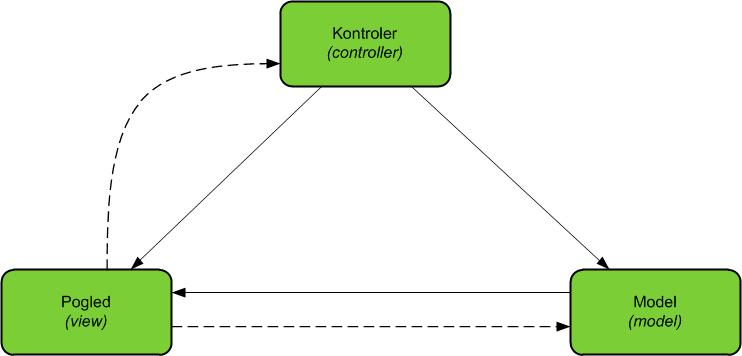
\includegraphics[width=0.6\linewidth]{django.jpeg}
\caption*{\textsl{Slika 1. Koncept modela MVC }}
\end{figure}
Pune linije predstavljaju vezu izmedju navedenih elemenata za razmenu podataka, dok isprekidane linije predstavljaju vezu kod koje neki drugi objekt vrši tu funkciju. Django koristi drugačije nazive elemenata MVC-a. Tako \textsl{view} predstavlja kontroler, a \textsl{template} (šablon) predstavlja \textsl{view} iz MVC-a pa implementaciju MVC-a možem za Django zvati kao MTV (\textsl{model-template-view}).  Ova promena je objašnjena na takav način što kod Djanga pogled predstavlja podatke koji se prezentuju dok šablon način na koji se podaci prikazuju. 

Model je zadužen za komunikaciju sa bazom podataka. Model je u Django okruženju klasa(engl. \textsl{class}) i određuje varijable i metode pridružene određenim tipovima podata. Pridružene varijable predstavljaju kolone u tablici dok metode definišu relacije između varijabli.  Ulog modela je da dohvati tražene podatke i prosledi ih ka pogledu.  Model nema informacija o šablonima i funkcijama izvedenih u pogledima. 

Uloga pogleda je prikazivanje podataka dohvaćenih iz baze podataka u internet pretraživaču. Priliko izrade web stranice, svaka kreirana aplikacija ima svoj pogled.  Pogled u stvari sačinjavaju funckije u Pytho programskom jeziku.  Ove funkcije imaju ulogu prenosnika podataka koji će biti prikazani.  

Pregled je HTML stranica s dodatnim strukturama koje omogućavaju prikaz podataka koji su poslati od pogleda.  Uloga pregleda je da sadržaj poslat od strane pogleda ugradi u HTML kod, koji će se prikazati u internet pretraživaču. 

\newpage
\section{Postupak za instaliranje}
\subsection{Instaliranje Python3 verzije }
Django je pisan u Python-u i kako bi ga koristili potrebno je imati instaliran Python. Python kao programski jezik postoji za sve tri popularne sistemske platforme Windows, Linux i OSX. Ovde će biti prikazan postupak instaliranja potrebnih paketa za rad pod Linux operativnim sistemom. Gotov sve distibucije linuxa dolaze sa instaliranim Python-om, razlika može biti u verziji. Postoje dve verzije, starija 2.7 verzija koja je podržana do kraja 2020. godine, i novija verzija 3.6. U radu je korišćena verzija 3.5. Proveru verzije radimo tako što otvorimo terminal i kucamo sledeću komandu : 
\begin{lstlisting}
 python3 --version
\end{lstlisting}
Ukoliko je Python verzije 3.6 instaliran, pojavi se sledeće
\begin{lstlisting}
 Python 3.6.6
\end{lstlisting}
\begin{figure}[h!]
\centering
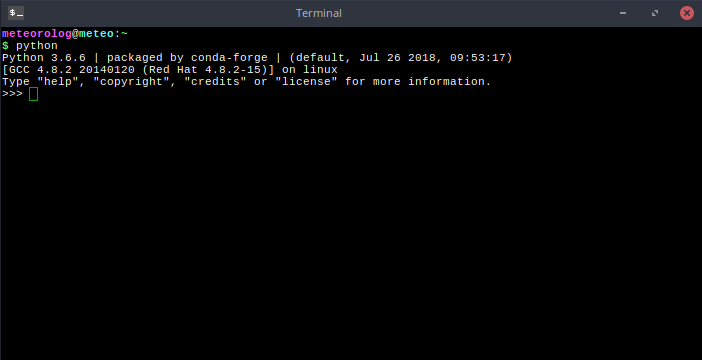
\includegraphics[width=1.\linewidth]{python.png}
\caption*{\textsl{Slika 2. Python verzije 3.6 pokrenut iz terminala}}
\end{figure}
Ukoliko nemate instaliran Python verzije 3.6, možete ga instalirati :
\begin{lstlisting}[language=Python]
 sudo apt install python3.6
 sudo dnf install python3
 sudo zypper install python3
\end{lstlisting}
gde je prva komanda za Debian, Fedoru i openSuse redom.
\subsection{Podešavanje virtuelnog okruženja}
Pre nego što instaliramo Django pokazaćemo kako instalirati veoma zahvalnu alatku, koja nam omogućava održavanje čistoće paketa na sistemu. Virtuelno okruženje (engl. \textsl{virtual environment}) izoluje projekte jedan od drugog, držeći pakete vezane za svaki projekat zasebno. Kako bi kreirali virtuelno okruženje zvano \textsl{env}, u direktorijum u kome smo započeli projekat, u terminal kucamo :
\begin{lstlisting}
 python3 -m virtualenv env
\end{lstlisting} [language=bash]
Kada ovo odradimo, u dokumentu se pojavi dokument \textsl{env} u koji će se instalirati svi paketi koje u buduće budemo koristili. Kada ovo sve odradimo, ostalo nam je još da ovo virtuelno okruženje aktiviramo. Aktiviranje virtuelno okruženja radimo na sledeći način :
\begin{lstlisting}
 source env/bin/activate
\end{lstlisting} 
nako čega se u terminalu pojavljuje nastavak \textsl{(env)}. Ovaj nastavak nam potvrđuje da je virtuelno okruženje aktvirano. Kako bi zatvorili virtuelno okruženje, u terminal kucamo komandu \textsl{deactivate}. 
\begin{figure}[h!]
\centering
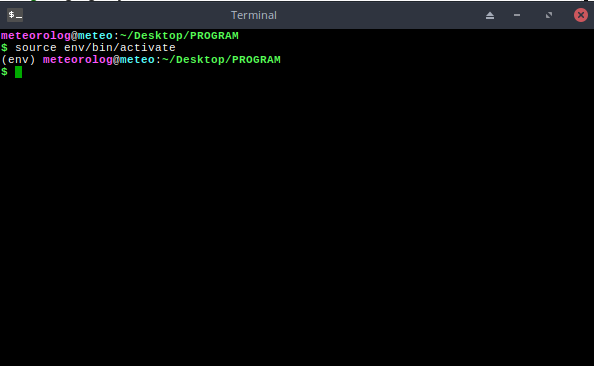
\includegraphics[width=1.\linewidth]{env.png}
\caption*{\textsl{Slika 3. Postupak aktiviranje virtuelnog okruženja}}
\end{figure}

\subsection{Instaliranje Djanga}
Kada smo podesili virtuelno okruženje možemo instalirati Django.  Instaliranje radimo pomoću  \textsl{Python Package Manager - pip}. Prvo uradimo nadogradnju pip paketa, kako bi imali poslednju verziju. To radimo na sledeći način :
\begin{lstlisting}
 (env)$ python3 -m pip install --upgrade pip
\end{lstlisting} 
Kada smo uradili nadogradnju pip-a, Django instaliramo :

\begin{lstlisting}
 pip install Django
\end{lstlisting} 
Kada ovo odradimo možemo uspešno pokrenuti naš prvi Django projekat.
\end{document}
